%!TEX root = geometry.tex
\stepcounter{lecture}
\setcounter{lecture}{2}
\sektion{Spherical geometry}

\subsection{Basics} % (fold)
\label{sub:basics}

\begin{definition}
	The {sphere $S^{\,2}$} is
	\begin{equation*}
		\left\{ (x,y,z) \subseteq \R^3 : x^2 + y^2 + z^2 = 1 \right\}.
	\end{equation*}
	The \emph{tangent space} to $S^{\,2}$ at $\pp\in S^{\,2}$ is
	\begin{equation*}
		T_{\pp}S^{\,2} = \pp^\perp \subseteq \R^3,
	\end{equation*}
	which is a vector space.
	% \missingfigure{Geo 4/1}
\end{definition}

The name tangent space is natural, because tangents to paths on the sphere naturally lie in this space:

\begin{proposition}
	If $\gamma:[0,1]\to S^{\,2}$ has $\gamma(t_0)=\pp$, then $\gamma\p(t_0) \in T_{\pp}S^{\,2}$ %
\end{proposition}

\begin{proof}
	We have $\gamma(t_0) \cdot \gamma(t_0) = 1$, so differentiating gives $2\,\gamma\p(t_0) \cdot \gamma(t_0) = 0$. Thus $\gamma\p(t_0) \perp \gamma(t_0)$. %
\end{proof}

\begin{definition}
	Points $\xx,-\xx \in S^{\,2}$ are called \emph{antipodal}. Antipodal points are diametrically opposite on the sphere. %
\end{definition}

We now consider some of the structures that we're used to in Euclidean geometry, and how they apply to the sphere. Lines are slightly different to those in $\R^3$:

\begin{definition}
	A line $L\subseteq S^{\,2}$ is $H\cap S^{\,2}$, where $H$ is a two-dimensional linear subspace (a plane) in $\R^3$ that passes through the origin.
\end{definition}

Some properties of lines on the sphere carry over nicely from Euclidean space. For example, the fact that (almost) any two points define a unique line:

\begin{proposition}
	There is a unique line through any two distinct, non antipodal points. %
\end{proposition}

\begin{proof}
	There's a unique plane in $\R^3$ containing any two linearly independent vectors. This generates our unique line. %
\end{proof}

We require that the two points not be antipodal, because otherwise we can define a family on lines of $S^{\,2}$, all from the family of planes in $\R^3$ that contain the line segment which joins them.

A concept that doesn't carry over from Euclidean geometry is that of parallel lines. In spherical geometry, these don't exist:

\begin{proposition}
	Any two distinct lines intersect in two antipodal points. %
\end{proposition}

\begin{proof}
	Any two distinct planes in $\R^3$ intersect in a one-dimensional linear subspace $\left\langle \vv \right\rangle$, which intersects $S^{\,2}$ in $\vv/\norm{\vv}$, $-\vv/\norm{\vv}$. %
\end{proof}

We can also think of spherical lines as circles in Euclidean space, centred at the origin, which have radius $1$.

	\pagebreak

Now we consider direction vectors on the sphere.

\begin{proposition}
	There exists a bijection %
	\begin{equation*}
		\left\{\text{lines $L$ passing through $\pp$}\right\}
		\longleftrightarrow
		\left\{ \vv \in T_{\pp} S^{\,2} : \vv \neq 0\right\} /
		\vv \sim \lambda \vv, \lambda\iR.
	\end{equation*}
\end{proposition}

\begin{proof}
	We construct our bijection as follows: %
	\begin{align*}
		L = H \cap S^{\,2} & \longrightarrow \pp^\perp \cap H = \left\langle \vv \right\rangle, \\
		\left\langle \vv,\pp \right\rangle & \longleftarrow \vv.
	\end{align*}
	This is a two-dimensional space, since $\vv\in\pp^\perp.$
\end{proof}

Our concepts of rays and line segments carry over nicely from Euclidean space:

\begin{definition}
	The \emph{ray} at $\xx$ = $(L,\vv)$ is one such that that $L$ is a line through $\xx$, with direction vector $\vv$ for $L$ at $\xx$ with $\norm{\vv}=1$.
	
	% \missingfigure{Geo 4/2}
	
	The \emph{line segment} from $\pp$ to $\qq$ is the shorter arc of the line joining $\pp$ and $\qq$.

	% \missingfigure{Geo 4/3}
	
	There is no unique line segment from $\pp$ to $\qq$ if $\pp$ and $\qq$ are antipodal.
\end{definition}

Similarly, if we think of angles as arising from our definition of scalar product, then our definition is the obvious one:

\begin{definition}
	If $(L_1,\vv_1)$ and $(L_2,\vv_2)$ are rays at $\xx$, then their \emph{angle} is the Euclidean angle
	\begin{equation*}
		\angle \vv_1,\vv_2 = \cos^{-1}\left( \f{\vv_1 \cdot \vv_2}{\norm{\vv_1} \norm{\vv_2}} \right).
	\end{equation*}
	% \missingfigure{Geo 4/4}
\end{definition}

Finally, we come to our notion of distance. We define it in the obvious way:

\begin{definition}
	If $\pp,\qq$ are non antipodal points on $S^{\,2}$, then the distance between them is given by
	\begin{equation*}
		d(\pp,\qq) = \text{length of line segment from $\pp$ to $\qq$} = \theta,
	\end{equation*}
	where $\theta=\angle \pp,\qq = \cos^{-1}(\pp\cdot\qq)$.

	If $\pp$ and $\qq$ are antipodal; that is, if $\qq=-\pp$, the $d(\pp,\qq) = \theta$.
	% \missingfigure{Geo 4/5}
\end{definition}

Now we need to show that this definition of distance turns the sphere into a metric space, because then a lot of nice properties follow easily.

We need to check the three conditions for a metric:
\begin{enumerate}
	\shortskip
	\item $d(\pp,\qq) = 0 \iff \pp=\qq$ (easy);
	\item $d(\pp,\qq) = d(\qq,\pp)$ (easy);
	\item The triangle inequality: $d(\pp,\qq) + d(\qq,\rr) \geq d(\pp,\rr)$.
\end{enumerate}
As is usually the case, checking the triangle inequality will be the hardest of the three. The best way to check this is to do some spherical trigonometry.

% subsection basics (end)

	\pagebreak

\subsection{Spherical trigonometry} % (fold)
\label{sub:spherical_trigonometry}

First we will need the following lemma:

\begin{lemma}
	If $\va,\vb,\vc \iR^3$, then \label{lem:spher-trig} %
	\begin{enumerate}
		\shortskip
		\item $\left( \va\cross\vc \right) \cdot \left( \vb\cross\vc \right) = \left( \vc\cdot\vc \right) \left( \va\cdot\vb \right) - \left( \va\cdot\vc \right)\left( \vb\cdot\vc \right)$; %
		\item $\left( \va\cross\vc \right) \cross \left( \vb\cross\vc \right) = \left( \left( \va\cross\vb \right) \cdot \vc \right) \vc$. %
	\end{enumerate}
\end{lemma}

\begin{proof}
	We can prove this in generality using suffix notation and the summation convention. Recall from \emph{Vectors \& Matrices} that
	\begin{equation*}
		\left( \va \cross \vb \right)_i = \epsilon_{ijk} a_j b_k
		\qquad \text{and} \qquad
		\epsilon_{ijk} \epsilon_{ilm} = \delta_{jl} \delta_{km} - \delta_{jm} \delta_{kl}.
	\end{equation*}
	With those in hand, we just expand the expressions accordingly:
	\begin{enumerate}
		\item \(\begin{aligned}[t]
			\left( \va \cross \vc \right) \cdot \left( \vb \cross \vc \right)
			&= \left( \va \cross \vc \right)_i \left( \vb \cross \vc \right)_i \\
			&= \epsilon_{ijk} a_j c_k \epsilon_{ilm} b_l c_m \\
			&= \left( \delta_{jl} \delta_{km} - \delta_{jm} \delta_{kl} \right) a_j c_k b_l c_m \\
			&= a_j c_k b_j c_k - a_j c_k b_k c_j \\
			&= \left( \vc\cdot\vc \right)\left( \va\cdot\vb \right) - \left( \va\cdot\vc \right)\left( \vb\cdot\vc \right).
		\end{aligned}\)
		\item \(\begin{aligned}[t]
			\left[ \left( \va\cross\vc \right) \cross \left( \vb\cross\vc \right) \right]_i
			&= \epsilon_{ijk} \left( \va\cross \vc \right)_j \left( \vb\cross\vc \right)_k \\
			&= \epsilon_{ijk} \epsilon_{jlm} a_l c_m \epsilon_{kpq} b_p c_q \\
			&= \epsilon_{kpq} \left( \delta_{kl} \delta_{im} - \delta_{km} \delta_{il} \right) a_l c_m b_p c_q \\
			&= \epsilon_{kpq} a_k c_i b_p c_q - \epsilon_{kpq} a_i c_k b_p c_q \\
			&= \left( \va\cross\vb \right)_q c_q c_i - \left( \vc\cross\vc \right)_p b_p a_i \\
			&= \left[ \left( \va\cross\vb \right) \cdot \vc \right] c_i.
		\end{aligned}\)
	\end{enumerate}
	This proves the lemma, and gives us a lot of the machinery that we need to do spherical geometry.
\end{proof}

% \begin{proof}
% 	[Sketch proof] Both identities are lines in $\va$ and $\vb$. Now, (i) is symmetric under switching $\va$ and $\vb$; (ii) is antisymmetric; and both are symmetric under the operation $(\ii,\jj,\kk) \mapsto (\kk,\ii,\jj)$. %
	
% 	Thus, it is sufficient to check for $(\va,\vb,\vc) = (\ii,\jj,\kk)$. For example, consider $\va=\ii,\vb=\ii$ and $\va=\ii,\vb=\jj$. %
	
% 	For $\va=\ii,\vb=\jj$ and $\vc=x\,\ii+ y\,\jj + z\,\kk$, (i) becomes
% 	\begin{equation*}
% 		\left( \ii\cross\vc \right) \cdot \left( \,\jj\cross \vc \right) \stackrel{?}{=} \left( \vc\cdot\vc \right) \left( \ii\cdot\jj \right) - \left( \ii\cdot\vc \right)\left( \,\jj\cdot\vc \right). %
% 	\end{equation*}
% 	This reduces to
% 	\begin{equation*}
% 		\left( y\,\kk-z\,\jj \right) \cdot \left( x\,\kk+z\,\ii \right) = -xy = 0 - xy,
% 	\end{equation*}
% 	so it holds in this case.
	
% 	For $\va=\ii$, $\vb=\ii$, (i) becomes
% 	\begin{equation*}
% 		\left( \ii\cross\vc \right) \cdot \left( \,\ii\cross \vc \right) \stackrel{?}{=} \left( \vc\cdot\vc \right) \left( \ii\cdot \ii \right) - \left( \ii\cdot\vc \right)^2, %
% 	\end{equation*}
% 	which reduces to
% 	\begin{equation*}
% 		\left\vert y\,\kk+z\,\jj \right\vert^2 = x^2 + y^2 + z^2 - x^2,
% 	\end{equation*}
% 	which is true. We can do similar calculations for (ii). We could alternatively prove both identities using suffix notation. %
% \end{proof}

\lecturemarker{5}{4 Feb}
To use this lemma properly, we need to make sure we know what scalar and vector products mean in $S^{\,2}$. The scalar product is the same as in $\R^3$, and the vector (or cross) product is only slightly different:

\begin{definition}
	Let $L\subset S^{\,2} \cap H$ be a ray passing through $\xx$ with unit direction vector $\tt$, with $\xx$ perpendicular to $\tt$. If $\xx,\tt\in H$, then the \emph{cross product} $\xx \cross \tt$ is the unit vector perpendicular to $H$.
\end{definition}

Now if we have two rays through $\xx$ with directions $\tt_1, \tt_2$, then we have already defined the angle $\theta$ between them to satisfy
\begin{equation*}
	\cos \theta = \tt_1 \cdot \tt_2.
\end{equation*}
Now let $\nn_i = \xx \cross \tt_i$ be the unit normal to $H_i$. Then
\begin{align*}
	\nn_1 \cdot \nn_2
	&= \left( \xx\cross\tt_1 \right) \cdot \left( \xx\cross\tt_2 \right) \\
	&= \left( -1 \right)^2 \left[ \left( \tt_1\cdot\tt_2 \right)\left( \xx\cdot\xx \right) - \left( \tt_1 \cdot \xx \right) \left( \tt_2\cdot\xx \right) \right] \tag{by (i) in the lemma} \\ %
	&= \left( \tt_1 \cdot \tt_2 \right)1 - 0 = \tt_1 \cdot \tt_2.
\end{align*}
Hence $\nn_1 \cdot \nn_2 = \cos\theta$.

This makes some sort of intuitive sense. If we consider the plane on the page, $T_{\xx} S^{\,2}$, then the unit normals are just rotations by $\pi/2$. Then clearly the angle $\theta$ is preserved.

% \missingfigure{Geo 5/1}

	\pagebreak

Next we need to consider what triangles mean on a sphere.

Now suppose we have a spherical triangle with vertices $\AA,\BB,\CC\in S^{\,2}$, with no two antipodal, sides of length $a,b,c$, and angles $\alpha,\beta,\gamma$.

Since drawing spherical triangles in three dimensions is often difficult without losing clarity, we often use two-dimensional representations of the form below. This captures much of the information about the triangle, but it significantly easier to draw and understand. The curved arcs represent the spherical lines that define the triangle.

\begin{center}
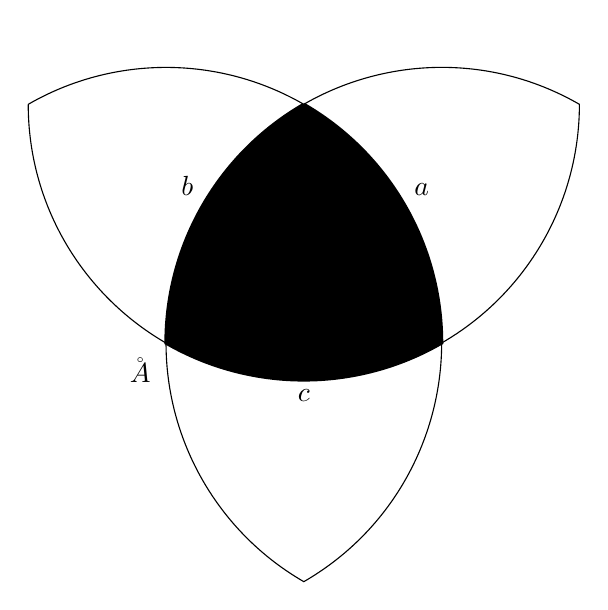
\begin{tikzpicture}[scale=3.5]
	
	\fill [fill=\shadeblack] (1,0) arc (60:0:1) arc (-60:-120:1) arc (180:120:1);

	\draw (0,0) arc (120:60:1)
					node [above=2pt] {$\CC$} arc (60:51:1)					% point C
					arc (-30:-150:0.15)
						arc (-150:-90:0.15) node [below] {$\gamma$}
						arc (-90:-30:0.15) arc (51:30:1)					% angle gamma
					node [above right] {$a$} arc (30:-60:1)					% distance a
				arc (240:180:1)
					node [below left=2pt] {$\AA$} arc (180:171:1)			% point A
					arc (90:-30:0.15)
						arc (-30:30:0.15) node [above right] {$\beta$}
						arc (30:90:0.15) arc (171:150:1)					% angle beta
					node [above left] {$b$} arc (150:60:1)					% distance b
				arc (0:-60:1)
					node [below right=2pt] {$\BB$} arc (-60:-69:1)			% point B
					arc (210:90:0.15)
						arc (90:150:0.15) node [above left] {$\alpha$}
						arc (150:210:0.15) arc (-69:-90:1)					% angle alpha
					node [below] {$c$} arc(-90:-180:1);						% distance x

	\draw [very thick] (1,0) arc (60:0:1) arc (-60:-120:1) arc (-180:-240:1);

\end{tikzpicture}
\end{center}

In particular, it's worth noting that $\alpha+\beta+\gamma>\pi$, as opposed to triangles in Euclidean space. We will explore the properties of angles of a spherical triangle in more detail later.

% \missingfigure{Geo 5/2}

Since the sides are given by arcs on a unit sphere, their lengths are just the angles that they span. Thus:
\begin{equation*}
	\cos a = \BB\cdot\CC, \qquad \cos b = \AA\cdot\CC, \qquad \cos c = \AA\cdot\BB.
\end{equation*}
Note that when we say $a$, $b$ and $c$ here, we really do mean the lengths, not the angles, since these lengths are actually angles.

% \missingfigure{Geo 5/3}

Now, if $\tt$ is the direction vector for the line segment pointing from $\AA$ to $\BB$, then
\begin{equation*}
	\AA\cross\BB = \sin c\,\nn_c = \sin c\left( \AA\cross\tt \right),
\end{equation*}
where $\nn_c$ is the unit normal to $\left\langle \AA,\BB \right\rangle$.

% \missingfigure{Geo 5/4}

	\pagebreak

\begin{proposition}
	Suppose we have a triangle on $S^{\,2}$ as described above. Then we have the following two rules, which are very similar to rules for triangles in $\Rn$. %
	\begin{enumerate}
		\item Cosine rule:
		\begin{equation*}
			\cos a = \cos b \cos c + \sin b \sin c \cos \alpha.
		\end{equation*}
		\item Sine rule:
		\begin{equation*}
			\f{\sin \alpha}{\sin a} = \f{\sin\beta}{\sin b} = \f{\sin\gamma}{\sin c}.
		\end{equation*}
	\end{enumerate}
\end{proposition}

\begin{proof}
	These follow very nicely from the machinery we derived in lemma~\ref{lem:spher-trig}. Consider:
	\begin{align*}
		\left( \AA\cross\BB \right) \cdot \left( \AA\cross\CC \right)
		&= \sin c \sin b \cos \alpha \\
		% \intertext{But this is also equal, by the lemma, to}
		&= \left( \BB\cdot \CC \right)\left( \AA\cdot\AA \right) - \left( \AA\cdot\BB \right)\left( \AA\cdot\CC \right) \\ %
		&= \left( \cos a \right)\cdot 1 - \cos b \cos c.
	\end{align*}
	Rearranging these gives the cosine rule.
	
	Now consider
	\begin{align*}
		\left( \AA\cross\BB \right) \cross \left( \AA\cross\CC \right)
		&= \sin c \sin b \left( \nn_c \cross \nn_b \right) \\
		&= \sin c \sin b \sin \alpha\,\AA. \\
		% \intertext{By the , this is also equal to}
		&= \left( \left( \AA\cross\BB \right)\cdot \CC \right) \AA \\
		&\Rightarrow \left( \AA\cross\BB \right)\cdot\CC = \sin c \sin b \sin\alpha.
	\end{align*}
	Now we know that this triple product is invariant under cyclic permutations, and so
	\begin{align*}
		\left( \AA\cross\BB \right)\cdot \CC &= \left( \CC\cross\AA \right)\cdot\BB \\
		\sin c\sin b\sin\alpha &= \sin b\sin a\sin\gamma.
	\end{align*}
	This second relation gives us
	\begin{equation*}
		\f{\sin\gamma}{\sin c} = \f{\sin\alpha}{\sin b},
	\end{equation*}
	and the rest of the rule follows by symmetry.
\end{proof}

	\vspace{3pt}

\begin{note}
	Suppose you're standing on the surface of the Earth. Technically, the Earth is approximately a sphere, but standing on its surface, the distances involved are so small that you might expect to be able to do plane geometry, and this turns out to be roughly right. We have $a,b,c\ll 1$. $\sin a \approx a$ and $\cos a \approx 1-a^2/2$. %

	The sine rule on spheres obviously reduces to the sine rule in the Euclidean plane. The cosine rule becomes
	\begin{equation*}
		(1-a^2/2) \approx (1-b^2/2) (1-c^2/2) + bc \cos \alpha,
	\end{equation*}
	which can be rearranged to give
	\begin{equation*}
		a^2 = b^2 + c^2 - 2bc \cos\alpha,
	\end{equation*}
	which is the cosine law in the plane.
\end{note}

% subsection spherical_trigonometry (end)

	\pagebreak

\subsection{Distance (again)} % (fold)
\label{sub:distance_again_}

Finally, we can return to where we started: trying to prove that our notion of distance defined a metric on the sphere, which required us to prove the triangle inequality. With a better understanding of spherical trigonometry, we can proceed.

\begin{corollary}
	[Triangle inequality] For points $\AA,\BB,\CC\in S^{\,2}$ and the distance function $d(\cdot,\cdot)$ as defined in section~\ref{sub:basics}, we have
	\begin{equation*}
		d(\BB,\AA) + d(\AA,\CC) \geq d(\BB,\CC),
	\end{equation*}
	with equality if and only if $\AA$ lies on the line segment $\BB\CC$ or $\BB$ and $\CC$ are antipodal. %
\end{corollary}

\begin{proof}
	Using the notation established in the previous section, we want to show that $c+b\geq a$. We know that
	\begin{align*}
		\cos\alpha
		&= \cos b \cos c + \sin b \sin c \cos \alpha \\
		&\geq \cos b \cos c - \sin b \sin c = \cos(b+c).
	\end{align*}
	Since $\cos$ is decreasing on $[0,\pi]$, we have $a\leq b+c$. %
\end{proof}

So now we have two metrics: the Euclidean metric $d_E$ on $\R^3$, and the spherical metric $d_S$ on $S^{\,2}$. It's natural to ask the following question:

If $\gamma:[0,1] \to S^{\,2} \subset \R^3$ is a path, and we define
\begin{itemize}
	\shortskip
	\item[] $L^E(\gamma) = \text{length of $\gamma$ with respect to the Euclidean metric on $\R^3$}$
	\item[] $L^S(\gamma) = \text{length of $\gamma$ with respect to the spherical metric}$
\end{itemize}
Are these two distances the same? It turns out that they are, which justifies our choice of spherical metric.

\begin{proposition}
	$L^E(\gamma) = L^S(\gamma)$. %
\end{proposition}

\begin{proof}
	Let $\pp$ and $\qq$ be two points on $S^{\,2}$, with an angle of $2\theta$ between their position vectors

	\begin{center}
		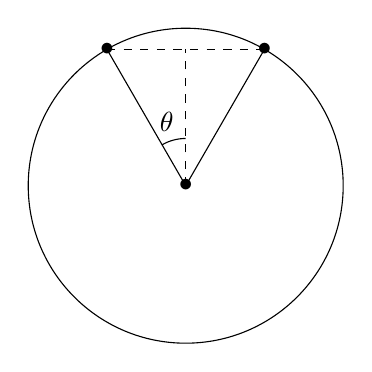
\begin{tikzpicture}[scale=2]
			\draw (0,0) circle (1);

			\draw (0,0) -- (-0.5,0.866) node [above left] {$\pp$};
			\draw (0,0) -- (0.5,0.866) node [above right] {$\qq$};

			\foreach \s in {-0.5, 0.5}
			{
				\draw (\s,0.866) node {$\bullet$};
			}

			\draw (0,0) node {$\bullet$};

			\draw [dashed] (0,0) -- (0,0.866);
			\draw [dashed] (-0.5,0.866) -- (0.5,0.866);
			\draw (0,0.3) arc (90:120:0.3);
			\draw (-0.12,0.28) node [above] {$\theta$};
		\end{tikzpicture}
	\end{center}

	Simple plane geometry tells us that $d_S(\pp,\qq) = 2\theta$ and $d_E(\pp,\qq) = 2\sin\theta$. Consider
	\begin{equation*}
		\lim_{\theta\to0} \f{d_S(\pp,\qq)}{d_E(\pp,\qq)} = \lim_{\theta \to 0} \f{\theta}{\sin\theta} = 1.
	\end{equation*}
	Given $\epsilon>0$, there is some $\delta_1>0$ such that if $d_E(\pp,\qq) < \delta_1$,
	\begin{equation*}
		d_E(\pp,\qq) \leq d_S(\pp,\qq) \leq \left( 1+\epsilon \right) d_E(\pp,\qq).
		\tag{$*$}
	\end{equation*}
	Since $\gamma$ is uniformly continuous, there is some $\delta_2>0$ such that
	\begin{equation*}
		d_E(\gamma(t),\gamma(s)) < \delta_1 \text{ whenever } \left\vert t-s \right\vert<\delta_2.
	\end{equation*}
	Now we consider the set of dissections
	\begin{equation*}
		D_\delta = \left\{A = \left\{0=t_0 < t_1 < \ldots < t_n = 1\right\} \mid t_i - t_{i-1} < \delta \;\forall i\right\} %
	\end{equation*}
	and this means we can write
	\begin{equation*}
		L(\gamma) = \sup_A L_A(\gamma) = \sup_A \left\{L_A(\gamma) \mid A\in D_\delta\right\}.
	\end{equation*}
	Then $(*)$ implies that if $A\in D_{\delta_2}$, then
	\begin{equation*}
		L_A^E(\gamma) \leq L_A^S(\gamma) \leq \left( 1+\epsilon \right) L_A^E(\gamma). %
	\end{equation*}
	Finally, for all $\epsilon>0$, we have
	\begin{equation*}
		L^E(\gamma) \leq L^S(\gamma) \leq \left( 1+\epsilon \right) L^E(\gamma),
	\end{equation*}
	and so $L^E(\gamma) = L^S(\gamma)$. %
\end{proof}

This is extremely useful, because it means we can use whichever metric is more convenient.

% subsection distance_again_ (end)

\subsection{Isometries} % (fold)
\label{sub:spherical_isometries}

Now we consider the isometries of the sphere. This will turn out to be easier than when we were working in $\Rn$. Let's start by considering orthogonal matrices:

\begin{example}
	Suppose $O\in O(3)$. If $\AA,\BB\in S^{\,2}$, then
	\begin{equation*}
		d(\AA,\BB) = \cos^{-1} (\AA\cdot\BB) = \cos^{-1}(O\AA \cdot O\BB) = d(O\AA, O\BB),
	\end{equation*}
	and so $O\in\Isom(S^{\,2})$. %
\end{example}

It turns out that these actually define all the isometries of the sphere:

\begin{theorem}
	$\Isom(S^{\,2}) = O(3)$. %
\end{theorem}

Remember how we showed this in the Euclidean case. We proved it with a series of lemmas. First we showed that if an isometry fixes the origin and the standard basis, then it is the identity. Again:

\begin{lemma}
	If $\phi\in\Isom(S^{\,2})$, $\phi(\ee_i) = \ee_i$ for $i=1,2,3$, then $\phi=\id_{S^{\,2}}$. %
\end{lemma}

\begin{proof}
	Let $\xx=(x_1,x_2,x_3)$, and $\phi(\xx)=\yy=(y_1,y_2,y_3)$. Then
	\begin{equation*}
		x_i
		= \xx\cdot\ee_i
		= \cos d(\xx,\ee_i)
		= \cos d(\phi(\xx), \phi(\ee_i)) = \cos(d(\yy,\ee_i))
		= \yy\cdot\ee_i = y_i.
	\end{equation*}
	Thus $x_i=y_i$ for $i=1,2,3$, and hence $\xx=\phi(\xx)$. %
\end{proof}

	\pagebreak

Notice that this was easier than the Euclidean case. Since we don't have translations on $S^{\,2}$, that's all we need to prove the theorem:

\begin{proof}
	[Proof of theorem] If $\phi\in\Isom(S^{\,2})$, then let $\vv_i = \phi(\ee_i)$. Then
	\begin{equation*}
		\vv_i \cdot \vv_j = \cos d(\vv_i,\vv_j) = \cos d(\ee_i,\ee_j) = \ee_i \cdot \ee_j = \delta_{ij}. %
	\end{equation*}
	Thus we can construct a matrix $O=(\vv_1,\vv_2,\vv_3) \in O(3)$. Thus $O\in\Isom(S^{\,2})$, with $O(\ee_i) = \vv_i$.

	Now $O^{-1}\circ\phi \in \Isom(S^{\,2})$, with $(O^{-1}\circ \phi)(\ee_i) = O^{-1}(\vv_i) = \ee_i$, and so $O^{-1} \circ \phi = \id_{S^{\,2}}$ by the lemma. Hence $\phi=O$. %
\end{proof}

\lecturemarker{6}{6 Feb}
Now we know what the isometries of $S^{\,2}$ are, let's consider how their properties relate to those in Euclidean space. Suppose $L=S^{\,2}\cap H$ is a line through $\xx$ with unit direction $\tt\in T_\xx S^{\,2}$.

If $O\in O(3)$, then $OL = S^{\,2} \cap OH$ is a line through $O\xx$ with unit direction $O\tt$, since $O\tt \in OH$ and $O\tt \cdot O\xx = \tt \cdot \xx = 0$. Thus $O\tt \in T_{O\xx} S^{\,2}$.

From this observation we draw the immediate corollary:

\vspace{2pt}

\begin{corollary}
	Isometries of $S^{\,2}$ preserve angles. %
\end{corollary}

\begin{proof}
	If $R_1,R_2$ are rays at $\xx$ with direction vectors $\tt_1, \tt_2$, then $OR_1, OR_2$ have direction vectors $O\tt_1, O\tt_2$, and %
	\begin{equation*}
		\cos \angle R_1, R_2 = \tt_1 \cdot \tt_2 = O\tt_1 \cdot O\tt_2 = \cos \angle OR_1, OR_2,
	\end{equation*}
	since $O\in O(3)$. Thus angles are preserved.
\end{proof}

Another concept we can bring over from our work in $\R^2$ is that of orthogonal frames:

\begin{definition}
	An \emph{orthogonal} frame at $\xx\in S^{\,2}$ is an ordered pair of unit tangent vectors $(\tt_1,\tt_2)$ with $\tt_i \in T_\xx S^{\,2}$ and $\tt_1 \perp \tt_2$. %
	
	% \missingfigure{Geo 6/1}

	The \emph{standard frame} $F_0$ at $(0,0,1)$ is $(\ee_1,\ee_2)$. %
\end{definition}

Our results from the Euclidean plane carry over naturally:

\begin{corollary}
	If $F_1=(\tt_1^1,\tt_2^1)$ is an orthogonal frame at $\xx_1$, and $F_2=(\tt_1^2, \tt_2^2)$ is an orthogonal frame at $\xx_2$, then there is a unique $O\in\Isom(S^{\,2})$ with $O(F_1) = F_2$. %
\end{corollary}

\begin{proof}
	Observe that $\xx_1, \tt_1, \tt_2$ is an orthonormal basis for $\R^3$, so we construct $O_1 = (\xx_1,\tt_1,\tt_2) \in O(3)$. %

	Then $O_1(F_0)=F_1$. Define $O_2$ similarly. Then $(O_2 \circ O_1^{-1})(F_1) = O_2 (F_0) = F_2$.

	Uniqueness is immediate, since an element of $O(3)$ is determined by its action on the basis $\xx_1, \tt_1, \tt_2$. %
\end{proof}

% This property is very important, and we call spaces that satisfy it \emph{homogeneous spaces}. Both the Euclidean plane and the sphere are homogeneous spaces.\todo{What is the exact defn of a homogneous space?}

% subsection spherical_isometries (end)

	\pagebreak

\subsection{Angle defect} % (fold)
\label{sub:angle_defect}

Now we come to the first beautiful theorem of the course, involving the previously discussed angle formula for triangles.

\begin{definition}
	If $\triangle ABC$ is a spherical triangle with angles $\alpha,\beta,\gamma$, then the \emph{angle defect} of $ABC$ is defined as
	\begin{equation*}
		\defect(ABC) = \alpha+\beta+\gamma - \pi.
	\end{equation*} %
\end{definition}

\begin{theorem}
	For a triangle as described above,
	\begin{equation*}
		\defect(ABC) = \Area(\triangle ABC).
	\end{equation*}
\end{theorem}

\begin{proof}
	First let's consider two lines on the sphere. A pair of lines divide $S^{\,2}$ into four spherical sectors, and without loss of generality, suppose they intersect at the poles. (Compare them to slices of an orange.) Looking downward: %
	
	\begin{center}
		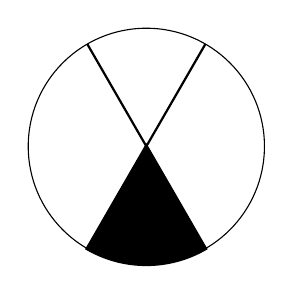
\begin{tikzpicture} [scale=1.5]
			\fill [fill=\shadeblack] (0,0) -- (0.5,-0.866025404) arc (-60:-120:1) -- cycle;

			\draw (0,0) circle (1);

			\draw [thick] (-0.5,0.866025404) -- (0.5,-0.866025404);
			\draw [thick] (-0.5,-0.866025404) -- (0.5,0.866025404);

			\draw [very thick] (0,0) -- (0.5,-0.866025404) arc (-60:-120:1) -- cycle;

			\draw (0,0) -- (0.1,-0.173205081) arc (-60:-120:0.2) -- cycle;
			\draw (0,-0.17) node [below=3pt] {$\Theta$};
		\end{tikzpicture}
	\end{center}

	Let $S_\Theta$ be the sector subtended by angle $\Theta$. Now $\Area(S^{\,2}) = 4\pi$, so $\Area(S_\Theta) = 2\Theta$, either by considering it as a proportion of the surface area of the whole sphere, or by considering the area integral %
	\begin{equation*}
		\Area(S_\Theta) = \int_{\theta=0}^{\Theta} \int_{\phi=-\pi/2}^{\pi/2} \sin\phi \dif{\theta} \dif{\phi}.	
	\end{equation*}
	A third line divides $S^{\,2}$ into an ``octahedron'' (strictly speaking, the projection of an octahedron onto a sphere). %
	
	% \missingfigure{Geo 6/3 -- these are an 90 degree angles, but we could easily  move them around}

	Consider the triangle $\triangle ABC$. This allows us to divide $S^{\,2}$ into two regions, $R$ and $-R$, where $R$ is $\triangle ABC$ and the three faces adjacent to $ABC$. We note that $-R$ is the image of $R$ under $\xx\mapsto-\xx$, so $\Area(R)=\Area(-R)$. Thus $\Area(R)=2\pi$.
	
	We label the triangles as follows (letting $\triangle 1 = \triangle ABC$):

	\begin{center}
	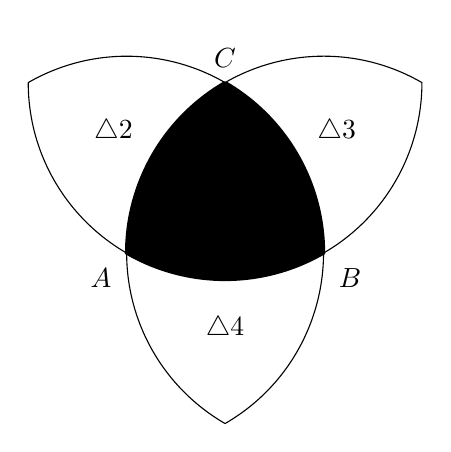
\begin{tikzpicture}[scale=2.5]
		
		\fill [fill=\shadeblack] (1,0) arc (60:0:1) arc (-60:-120:1) arc (180:120:1);
	
		\draw (0,0) arc (120:60:1)
						node [above=2pt] {$C$} arc (60:51:1)					% point C
						arc (-30:-150:0.15)
							arc (-150:-90:0.15) node [below] {$\gamma$}
							arc (-90:-30:0.15) arc (51:30:1)					% angle gamma
						node [above right] {} arc (30:-60:1)
					arc (240:180:1)
						node [below left=2pt] {$A$} arc (180:171:1)				% point A
						arc (90:-30:0.15)
							arc (-30:30:0.15) node [above right] {$\beta$}
							arc (30:90:0.15) arc (171:150:1)					% angle beta
						node [above left] {} arc (150:60:1)
					arc (0:-60:1)
						node [below right=2pt] {$B$} arc (-60:-69:1)			% point B
						arc (210:90:0.15)
							arc (90:150:0.15) node [above left] {$\alpha$}
							arc (150:210:0.15) arc (-69:-90:1)					% angle alpha
						node [below] {} arc(-90:-180:1);
	
		\draw [very thick] (1,0) arc (60:0:1) arc (-60:-120:1) arc (-180:-240:1);
	
		\draw (0.433012702,-0.25) node {$\triangle 2$};
		\draw (1.566987298,-0.25) node {$\triangle 3$};
		\draw (1,-1.25) node {$\triangle 4$};

	\end{tikzpicture}
	\end{center}

	Now we notice that pairs of triangles form spherical sectors:
	\begin{align*}
		1\cup 4 &= \text{spherical sector with $\angle\gamma$}, \\
		1\cup 3 &= \text{spherical sector with $\angle\alpha$}, \\
		1\cup 2 &= \text{spherical sector with $\angle\beta$}.
	\end{align*}
	Then using the previously discussed formula for the area of a spherical sector, we have
	\begin{align*}
		\Area(1\cup 4) &= 2\gamma, \\
		\Area(1\cup 3) &= 2\alpha, \\
		\Area(1\cup 2) &= 2\beta.
	\end{align*}
	We've already seen that $\Area(R)=2\pi$, and $R=1 \cup 2 \cup 3 \cup 4$. Thus
	\begin{equation*}
		2\pi
		= \Area(1 \cup 2 \cup 3 \cup 4)
		= 2\gamma + 2\alpha + 2\beta - 2\Area(1).
	\end{equation*}
	But $\Area(1)=\Area(\triangle ABC)$, and so rearranging just gives
	\begin{equation*}
		\Area(\triangle ABC) = \alpha+\beta+\gamma-\pi = \defect(ABC). \qedhere
	\end{equation*}
\end{proof}

Now let's look at an application of this.

\begin{definition}
	A \emph{spherical polyhedron $P$} is
	\begin{enumerate}
		\shortskip
		\item A set of points (vertices) in $S^{\,2}$;
		\item A set of line segments (edges) in $S^{\,2}$ which are disjoint except at vertices;
		\item Faces of $P$, the connected components $S^{\,2}-\{\text{edges}\}$.
		\item Every vertex lies on an edge.
	\end{enumerate}
\end{definition}

\begin{theorem}
	[Euler's formula] If $P$ is a spherical polyhedron with $V$ vertices, $E$ edges and $F$ faces, then %
	\begin{equation*}
		V-E+F=2.
	\end{equation*}
\end{theorem}

\begin{proof}
	Suppose some face has more than three sides. Then we can subdivide the face to make a new $P\p$ with $V\p=V$ vertices, $E\p=E+1$ edges and $F\p=F+1$ faces. Thus $V\p-E\p+F\p = V-E+F$. %
	
	\begin{center}
		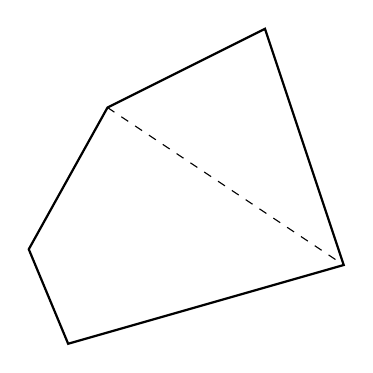
\begin{tikzpicture}
			\draw [thick] (0,0) -- (2,1) -- (3,-2) -- (-0.5,-3) -- (-1,-1.8) -- cycle;
			\draw [dashed] (0,0) -- (3,-2);
		\end{tikzpicture}
	\end{center}

	Thus, it is sufficient to prove Euler's formula for the subdivided shape. After repeated subdividing, we can assume that all faces are triangles. %

	Every triangle has three edges, and every edge borders two faces. Thus
	\begin{equation*}
		3F=2E \text{ or } E=\tf{3}{2}F. \tag{$*$}
	\end{equation*}
	Now consider the sum of the angles:
	\begin{align*}
		S
		&= \text{sum of every angle in every face of $P$} \\
		&= \text{sum of every angle at every vertex of $P$}.
	\end{align*}
	Working from the face-based definition, we have:
	\begin{equation*}
		S
		= \sum_{\text{faces $f$}} \sum_{\substack{\text{angles $\theta_i$} \\ \text{in $f$}}}
		= \sum_{\text{faces $f$}} \left[ \pi+\Area(f) \right]
		=\pi F + \Area(S^{\,2}) = \pi F + 4\pi.
	\end{equation*}
	Alternatively, using the vertex definition, we have
	\begin{equation*}
		S
		=\sum_{\text{vertices $v_i$}} \sum_{\substack{\text{angles $\theta_i$} \\ \text{at $v$}}}
		= \sum_v 2\pi = 2\pi V
	\end{equation*}
	Combining these, we have
	\begin{equation*}
		2\pi V = \pi F + 4\pi \implies F=2V-4. \tag{$**$}
	\end{equation*}
	Combining equations~($*$) and ($**$), we have
	\begin{equation*}
		V-E+F = V-\tf{1}{2}F = V-\tf{1}{2}\left( 2V-4 \right) = 2. \qedhere
	\end{equation*}
\end{proof}

Now let's recast this in a form we might be slightly more familiar with:

\begin{definition}
	A \emph{convex Euclidean polyhedron} is a convex bounded subset of $\R^3$ bounded by a finite number of planes. That is, %
	\begin{equation*}
		P = \bigcap_{i=1}^n X_i,
	\end{equation*}
	where $X_i = \left\{\xx\iR^3 : \xx\cdot \vv_i \leq c_i\right\}$.
\end{definition}

\begin{corollary}
	If $P$ is a convex Euclidean polyhedrom with $V$ vertices, $E$ edges and $F$ faces, then $V-E+F=2$. %
\end{corollary}

\begin{proof}
	After translation, we can assume that the origin is inside $P$. Then consider the map which projects $P$ on to the surface of the sphere.
	\begin{equation*}
		\fullfunction{\pi}{\R^3-O}{S^{\,2}}{\vv}{\vv/\norm{\vv}}
	\end{equation*}
	The image of $P$ is a spherical polyhedron $P\p$ with $V$ vertices, $E$ edges and $F$ faces. %

	Note that an edge of $P\p$ is a Euclidean line segment. It projects to the spherical line segment lying on $H$, where $H$ is the plane spanned by $O$ on $L$. %
\end{proof}

% subsection angle_defect (end)

	\pagebreak

\subsection{Topology of surfaces} % (fold)
\label{sub:topology_of_surfaces}

\newcommand{\biggarrow}{\draw [decoration={markings,mark=at position 1 with {\arrow[scale=2]{>>}}},
    		   postaction={decorate},
    		   shorten >=0.4pt]}

\lecturemarker{7}{11 Feb}
\begin{definition}
	A \emph{surface} is a metric space $S$ which is locally homeomorphic to $\R^2$; that is, for every $\xx\in S$, there's an open $U\ni x$ and a homeomorphism
	\begin{equation*}
		\phi_U: U\to B_0(1) = \left\{ \xx\iR^2 : \vvert{\xx} < 1 \right\}.
	\end{equation*}
\end{definition}

Notice that there's nothing special about $2$ in this definition. If we replace $2$ by $n$, then we recover the definition of an \emph{$n$-dimensional manifold}. We will study these objects further in Part~II. 

\begin{examples}
\mbox{}
\begin{enumerate}
	\item Trivially, $\R^2$.
	\item The sphere $S^{\,2}$. Given $\xx\in S^{\,2}$, take $U_\xx$ to be the open hemisphere which contains $\xx$. Let $\phi_{U_\xx}$ be the projection on to the plane which cuts out the hemisphere.

	\begin{center}
		\begin{tikzpicture} [scale=1.8]

			\fill [\shadeblack] (0,0) -- (50:1) arc (50:230:1) -- cycle;

			\draw (0,0) ++ (140:0.45) node {$U_\xx$};

			\draw [thick] (0,0) circle (1);
			\draw (0,0) node {$\bullet$};

			\draw (0,0) ++ (140:1) node {$\bullet$};
			\draw (0,0) ++ (140:1) node [above left] {$\xx$};

			\draw [dashed] (0,0) -- (50:1.5);
			\draw [dashed] (0,0) -- (-130:1.5);
		\end{tikzpicture}
	\end{center}

	In the diagram above, we consider a cross-section of the sphere. The hemisphere containing $\xx$ is shaded, and we project onto the dashed line (the plane which removes $U_\xx$ from $S^{\,2}$). We will see a form of this later, when we discuss \emph{stereographic projections.}
	\item The cylinder $S^{\,1} \times \R = (\R/\Z) \times \R = \R^2/\Z$, where $\Z\cong \left\langle \left( 1,0 \right) \right\rangle \subset \R^2$.

	\begin{center} % Geo 7/1 
		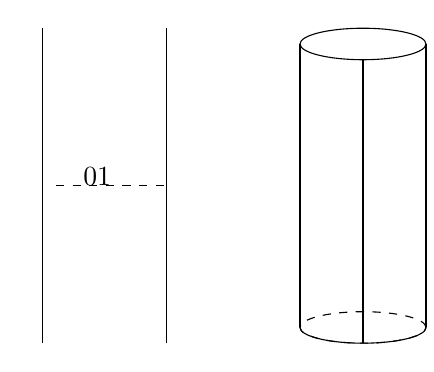
\begin{tikzpicture}

			\foreach \s in {0,1} {
				\bigarrow (-0.7+\s*1.4,-2) node [below=2pt] {$\s$} -- ++ (0,2.8);
				\draw (-0.7+\s*1.4,-2) -- ++ (0,4);
			}

			\draw [dashed] (-0.7,0) -- (0.7,0);
			\biggarrow (-0.2,0) -- (0,0);

			\foreach \s in {-1,1} {\draw (3.2,\s*1.8) circle (0.8 and 0.2);}

			\biggarrow (3.5,1.61) -- (3.6,1.615);

			\fill [white] (2,-1.8) rectangle (4.1,-1.5);
			\draw [dashed] (3.2,-1.8) circle (0.8 and 0.2);

			\draw (3.2,-2) -- (3.2,1.6);

			\foreach \s in {2.4,4} {\draw (\s,1.8) -- (\s,-1.8);}

		\end{tikzpicture}
	\end{center}

	The diagram above shows that the cylinder can also be thought of as $[0,1] \times \R$. We take a pair of infinite lines at $0$ and $1$ (left), and we wrap them around until they meet, and this is the infinite cylinder (right). The interval $[0,1]$ is mapped to a circle, which we recover by taking a cross-section of the cylinder.

		\pagebreak

	\item Möbius band, $M=[0,1] \times [-1/1] / \sim$, where $(0,y) \sim (1,-y)$.

	\vspace{6pt}

	% Preamble for the Möbius strip
	% Taken from Möbius.tex

	% one third of the Moebius Strip
	%: \strip{<angle>}
	\newcommand{\strip}[1]{%
	\shadedraw[thick,top color=white,bottom color=gray, rotate=#1]
	 (0:2.8453) ++ (-30:1.5359) arc (60:0:2)
	 -- ++  (90:5) arc (0:60:2) -- ++ (150:3) arc (60:120:2) 
	 -- ++ (210:5) arc (120:60:2) -- cycle;}

	%: \MoebiusStrip{<text1>}{<text2>}{<text3>}
	\newcommand{\MoebiusStrip}[3]{%
	\begin{scope} [transform shape]
		\strip{0}
		\strip{120}
		\strip{-120}
		\draw (-60:3.5) node[scale=6,rotate=30] {#1};
		\draw (180:3.5) node[scale=4,rotate=-90]{#3};
		% redraw the first strip after clipping
		\clip (-1.4,2.4)--(-.3,6.1)--(1.3,6.1)--(5.3,3.7)--(5.3,-2.7)--cycle;
		\strip{0}
		\draw (60:3.5) node [gray,xscale=-4,yscale=4,rotate=30]{#2};
	\end{scope}}

	% \include{Möbius.tex}
	\begin{minipage}{0.55\textwidth}
		\centering
		\begin{tikzpicture}[xscale=2,yscale=2]
			\draw (-1,0) rectangle (1,1);

			\foreach \s in {-1,1} {\bigarrow (\s,0) -- (\s,0.55);}

			\foreach \s/\t/\u in {-1/0/below left, -1/1/above left, 1/0/below right, 1/1/above right}
			{\draw (\s,\t) node [\u] {$(\s,\t)$};}

		\end{tikzpicture}
	\end{minipage}
	\hspace{0.3cm}
	\begin{minipage}{0.35\textwidth}
		\begin{tikzpicture} [rotate=22,scale=0.25]
			\MoebiusStrip{}{}{}
		\end{tikzpicture}
	\end{minipage}

	\vspace{6pt}

	Traditionally we make a Möbius band by taking a strip of paper, twisting one end and glueing the ends together. Geometrically, we take the rectangle $[0,1] \times [-1/1]$ with a specified orientation, and we join the ends together in such a way that preserves orientation.

	In the diagram above, we have included several arrows to better illustrate how orientation is preserved.

	\emph{The TikZ code for the shaded Möbius strip was written by Jacques~Duma and Gerard~Tisseau, published online at \href{http://math.et.info.free.fr/TikZ/index.html}{http://math.et.info.free.fr/TikZ/index.html}.}
	
	\item The torus $T^2 = S^{\,1} \times S^{\,1} = (\R/\Z) \times (\R/\Z) = \R^2/\Z^2$.

	Constructing a torus from elementary geometry is slightly, but not significantly, more difficult than anything we've done so far. First consider the rectangle $\left[ 0,1 \right]^2$, with a clockwise orientation:

	\begin{center} % Geo 7/3 
		\begin{tikzpicture}[scale=2.25]

			% Square

			\draw (0,0) rectangle (1,1);

			\foreach \s/\t/\u in {0/0/below left, 0/1/above left, 1/0/below right, 1/1/above right}
			{\draw (\s,\t) node [\u] {$(\s,\t)$};}

			\foreach \s in {0,1} {
				\bigarrow (0,\s) -- (0.5,\s);
				\biggarrow (\s,0) -- (\s,0.6);
			}

			% Cylinder

			\foreach \s in {-1,1} {\draw [thick] (3,0.5+\s*0.9) circle (0.4 and 0.1);}

			\bigarrow [thick] (3.15,1.31) -- (3.2,1.315);

			\fill [white] (2.5,-0.4) rectangle (3.5,-0.25);
			\draw [dashed, thick] (3,-0.4) circle (0.4 and 0.1);

			\draw (3,1.3) -- (3,-0.5);

			\foreach \s in {2.6,3.4} {\draw (\s,1.4) -- (\s,-0.4);}

			\bigarrow [thick] (2.85,-0.49) -- (2.8,-0.485);
		\end{tikzpicture}
	\end{center}

	We wrap this around to construct a cylinder, not unlike example~(iii). However, this is finite in both dimensions. Notice that the orientation in the two circular faces go in the opposite directions.

	% We say that $[0,1] \times [0,1]$ is a \emph{fundamental domain} factorisation of $\Z^2$; that is, it’s closed, and every point in $\R^2$ is equivalent to some point in it. % (Consider that we say in \emph{Numbers \& Sets} that $[0,1]$ and $\R$ have the same cardinality; it intuitively follows that there is an equivalence between $\left[ 0,1 \right]^2$ and $\R^2$.)

	\begin{center}
		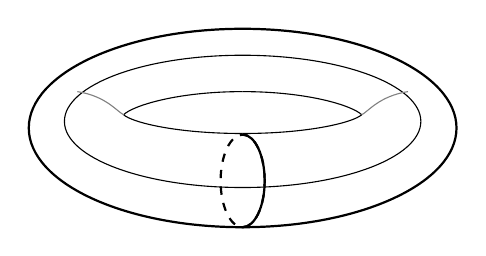
\begin{tikzpicture} [scale=0.28, yscale=0.5]

			\draw [thick] (0,-4.8) circle (1 and 4.2);
			\fill [white] (0,-0) rectangle (-2,-9);
			\draw [thick, dashed] (0,-4.8) circle (1 and 4.2);

			\draw [thick] (0,0) circle (9.7 and 9);
			\draw (0,0.6) circle (8.0833 and 6);

			\draw (0,3.3) .. controls (3,3.3) and (5,2) .. (5.4,1.2);
			\draw (0,-0.5) .. controls (3,-0.5) and (5,0.5) .. (5.4,1.2);

			\draw (0,3.3) .. controls (-3,3.3) and (-5,2) .. (-5.4,1.2);
			\draw (0,-0.5) .. controls (-3,-0.5) and (-5,0.5) .. (-5.4,1.2);

			\draw [thin, gray] (5.4,1.2) .. controls (5.7,1.5) and (6.2,2.9) .. (7.5,3.3);
			\draw [thin, gray] (-5.4,1.2) .. controls (-5.7,1.5) and (-6.2,2.9) .. (-7.5,3.3);
		\end{tikzpicture}
	\end{center}

	Then we wrap the two ends of the cylinder around to make a torus, or a doughnut shape.

	There's nothing special about the $2$ in the definitions of $S^{\,2}$ and $T^{\,2}$. Both constructions are dimension independent; we can just as easily, for example, define $T^{\,7}$ embedded in $\R^7$.

	% 	\pagebreak

	% \item $\R P^2$, the real projective plane, which is given by $S^{\,2}/\sim$, with $\xx \sim -\xx$.

	% This is essentially the projection we saw in example~(i), with the point $\xx$ fixed at the north pole. To find the image $\pp\p$ of a point $\pp$, we draw the line

	% \begin{center}
	% 	\begin{tikzpicture} [scale=2]
	% 		\draw (0,0) circle (1);
	% 		\draw [dashed] (-2,0) -- (2,0);

	% 		\draw (0,1) node {$\bullet$};
	% 		\draw (0,1) ++ (-160:1) node {$\bullet$};

	% 		\draw (0,1) ++ (-160:1) node [below right] {$\pp$} -- (0,1) node [above=2pt] {$(0,0,1)$};
	% 	\end{tikzpicture}
	% \end{center}

	% \begin{remark}
	% 	There's \emph{no} subset of $\R^3$ homeomorphic to $\R P^2$. The fundamental domain is $\left\{(x,y,z) \in S^{\,2} : z\geq 0 \right\}$ is a closed hemisphere.

	% 	is $(x,y,z) \to (x,y)$.

	% 	$x^2+y^2+z^2=1$ so $z=\sqrt{1-x^2-y^2}$.

	% 	$(x,y,0) \sim (-x,-y,0)$

	% 	$\R P^2 = \overline{B}^{\,2} / \sim$. where $\xx\sim -\xx$ for $\xx\in S^{\,1}$.
	% 	\missingfigure{Geo 7/7}

	% 	$\R P^2 = [-1,1] \times [-1,1] / \backslash$
	% 	$(-1,y) \sim (1,-y)$
	% 	$(x,1) \sim (-x,-1)$

	% 	Another way to consider this, and to see that $\R P^2$ cannot be embedded in $\R^3$, is to consider that it is the Mobius band with its edge glued to itself.
	% 	\missingfigure{Geo 7/8}
	% 	This is clearly impossible.
	% \end{remark}
\end{enumerate}
\end{examples}

% \subsubsection*{Digression on progressive geometry} % (fold)
% \label{ssub:progression_on_projective_geometry}

% A line in $\R P^2$ is the image of a line in $S^{\,2}$.

% Now $L_1, L_2 \subset S^{\,2}$ intersect in two antipodal points.

% If $\pi:S^{\,2} \to \R P^2$. then $\pi(L_1), \pi(L_2)$ intersect in one point.

% There is a unique line between any two points.

% But: $\R P^2 - \pi(L)$ is $\stackrel{\circ}{B}^{\,2}$ (the open unit ball). For example, consider the $x,y$ plane intersected with $S^{\,2}$. This is connected. (Compare with the Euclidean plane; take away a line and get two different pieces.)

% subsubsection progression_on_projective_geometry (end)

% subsection topology_of_surfaces (end)

\subsection{Building surfaces} % (fold)
\label{sub:building_surfaces}

\begin{definition}
	Let $S_1$ and $S_2$ be surfaces, and $\phi_i:U_i \to B_0(1)$, where $U_i \subset S_i$.

	Then we define the \emph{connected sum of $S_1$ and $S_2$}, denoted $S_1 \# S_2$, to be
	\begin{equation*}
		S_1 \# S_2 = \left[ S_1 - \phi_1^{-1}(B_0(\tf{1}{2})) \right] \cup \left[ S_2 - \phi_2^{-1}(B_0(\tf{1}{2})) \right] / \sim,
	\end{equation*}
	where $\phi_1^{-1}(\tf{1}{2}z) \sim \phi_2^{-1}(\tf{1}{2}\overline{z})$ for $z\in S^{\,1}$.
\end{definition}

For example, we can connect two copies of $T^{\,2}$ in this way to construct a two-holed torus, which is a surface of genus $2$. Indeed, in general, a surface of genus $g$ is the connected sum of $g$ copies of $T^{\,2}$.

% In pictures:
% \missingfigure{Geo 7/9}
% This is a surface of genus 2.

% In general, a surface of genus $g$ is the connected sum of $g$ copies of $T^{\,2}$.
% \missingfigure{Geo 7/10}

\emph{Fact.} Every compact surface is one of
\begin{enumerate}
	\shortskip
	\item $S^{\,2}$;
	\item $\#^g T^{\,2}$ (a genus $g$ surface);
	\item $\#^n \R P^2$.
\end{enumerate}
We will study this further in Part~II \emph{Algebraic Geometry}.

This obviously doesn't work in higher dimensions. For example, there are infinitely many three-manifolds that are not decomposable as connected sums.

Now let's look at another way of building surfaces.

\begin{definition}
	A \emph{triangulated surface} is obtained by starting with a disjoint union of closed triangles and identifying pairs of edges. Each triangle will be embedded with an orientation, and we join them in such a way as to preserve orientation.

	\begin{minipage}{0.24\textwidth}
		\centering
		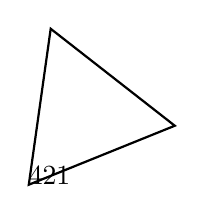
\begin{tikzpicture} [scale=2, rotate=22]
			\draw [thick] (0,0) -- (1,0) -- ++ (120:1) -- cycle;
			
			\bigarrow [thick] (0,0) -- (0.6,0) node [below=3pt] {$4$};
			\bigarrow [thick] (0,0) ++ (60:1) -- ++ (-60:0.6) node [above right=2pt] {$2$};
			\bigarrow [thick] (0,0) -- ++ (60:0.6) node [left=4pt] {$1$};
		\end{tikzpicture}
	\end{minipage}
	\begin{minipage}{0.24\textwidth}
		\centering
		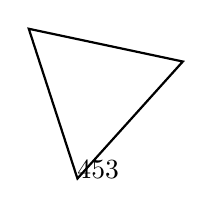
\begin{tikzpicture} [scale=2, rotate=48]
			\draw [thick] (0,0) -- (1,0) -- ++ (120:1) -- cycle;
			
			\bigarrow [thick] (0,0) -- (0.6,0) node [below right=1pt] {$4$};
			\bigarrow [thick] (1,0) -- ++ (120:0.5) node [above right=3pt] {$5$};
			\bigarrow [thick] (0,0) -- ++ (60:0.6) node [below left=3pt] {$3$};
		\end{tikzpicture}
	\end{minipage}
	\begin{minipage}{0.24\textwidth}
		\centering
		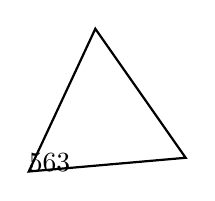
\begin{tikzpicture} [scale=2, rotate=5]
			\draw [thick] (0,0) -- (1,0) -- ++ (120:1) -- cycle;
			
			\bigarrow [thick] (0,0) -- (0.6,0) node [below=3pt] {$5$};
			\bigarrow [thick] (1,0) -- ++ (120:0.5) node [above right=3pt] {$6$};
			\bigarrow [thick] (0,0) -- ++ (60:0.6) node [left=4pt] {$3$};
		\end{tikzpicture}
	\end{minipage}
	\begin{minipage}{0.24\textwidth}
		\centering
		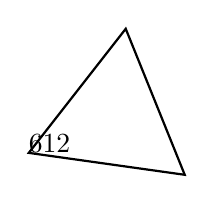
\begin{tikzpicture} [scale=2, rotate=-8]
			\draw [thick] (0,0) -- (1,0) -- ++ (120:1) -- cycle;
			
			\bigarrow [thick] (0,0) -- (0.6,0) node [below left=3pt] {$6$};
			\bigarrow [thick] (1,0) -- ++ (120:0.5) node [right=4pt] {$1$};
			\bigarrow [thick] (0,0) -- ++ (60:0.6) node [left=5pt] {$2$};
		\end{tikzpicture}
	\end{minipage}

	The result is a compact surface. (This means that is is bounded bounded and closed.)

	If $S$ is a triangulated surface with $V$ vertices, $E$ edges and $F$ faces, then
	\begin{equation*}
		\chi(S) = V-E+F
	\end{equation*}
	is the \emph{Euler characteristic} of $S$.
\end{definition}

Let's consider how we might go about computing this Euler characteristic. Counting the number of faces and edges is easily found from the number of triangles which we start with, but counting the number of vertices is more difficult.

Let's consider the Euler characteristic of a connected sum. If $S_1,S_2$ are triangulated surfaces, then we can make a triangulated surface homeomorphic to $S_1 \# S_2$ by removing one face from each of $S_1$ and $S_2$, and identifying edges of those faces. Thus
\begin{equation*}
	F_\# = F_1 + F_2 - 2, \qquad E_\# = E_1 + E_2 - 3, \qquad V_\# = V_1 + V_2 - 3.
\end{equation*}
Substituting into the definition of Euler characteristic, we have
\begin{equation*}
	\chi(S_1 \# S_2) = \chi(S_1) + \chi(S_2) - 2,
\end{equation*}
which gives us a good way to compute the Euler characteristic for complicated surfaces. If we can represent it as the connected sum of simpler surfaces of which we already know the Euler characteristic, then we can compute its Euler characteristic using the formula above.

If $S_1$ and $S_2$ are homeomorphic to one another, and in turn homeomorphic to $S^{\,2}$, then $\chi(S_1) = \chi(S_2)$, and so the Euler characteristic is a topological invariant. The basic idea is to construct triangulated surfaces on $S^{\,2}$ that are homeomorphic to $S_1$ and $S_2$, then apply the formula we already know for convex spherical polyhedra to them.

\begin{example}
	If we take a triangulation of a torus $T^2$, then it has Euler characteristic $0$ (unproved). Thus the connected sum of $g$ tori, a surface of genus $g$, has
	\begin{equation*}
		\chi(\#^g T^2) = 0 - 2\left( g-1 \right) = 2-2g.
	\end{equation*}
\end{example}

Finally, this example should make us wonder whether the Euler characteristic is well-defined for general surfaces, and not just triangulated ones. This turns out to be the case, although we won't prove it here; instead, see \emph{Algebraic Topology}.

% The basic idea of the proof is that if $S_1 \cong S_2 \cong S^{\,2}$, then given a triangulation of $S^{\,2}$, we can show that there's a spherical polyhedron with $F$ faces, $E+n$ edges and $V+n$ vertices. This is homeomorphic to $S_1$ and $S_2$, and then we use $V-E+F=2$ on spherical polyhedron.

% \missingfigure Geo 7/13

% \begin{remark}
% 	We should consider whether this characteristic is well-defined for general surfaces, not just triangulated ones. We won't prove it here; instead see \emph{Algebraic Topology}.
% \end{remark}

% subsection building_surfaces (end)